\documentclass{article}
\usepackage[cm]{fullpage}
\usepackage{graphicx}
\usepackage{hyperref}
\usepackage{natbib}
\usepackage{amsmath,amssymb}
\DeclareMathOperator*{\argmin}{arg\,min}
\DeclareMathOperator*{\Diag}{Diag}
\DeclareMathOperator*{\TPR}{TPR}
\DeclareMathOperator*{\FPR}{FPR}
\DeclareMathOperator*{\argmax}{arg\,max}
\DeclareMathOperator*{\maximize}{maximize}
\DeclareMathOperator*{\minimize}{minimize}
\newcommand{\RR}{\mathbb R}

\begin{document}

\title{Benchmarking fpop}
\author{Toby Dylan Hocking and Guillem Rigaill}
\maketitle

\tableofcontents

\section{Introduction}

fpop is a new segmentation algorithm that uses Functional Pruning and
Optimal Partitioning, proposed by Robert Maidstone, Guillem Rigaill
and Paul Fearnhead. The purpose of this report is to benchmark the
speed of the fpop algorithm. 

The algorithm is a solver for the penalized least squares segmentation
problem. Given $d$ ordered, noisy observations or data points
$\mathbf y = \left[
\begin{array}{ccc}
y_1 & \cdots & y_d  
\end{array}
\right]\in\RR^d $ and some positive penalty constant
$\beta\in\RR_+$, we want to find the piecewise constant mean vector
\begin{equation}
  \label{eq:ytilde^beta}
  \mathbf{\tilde y}^\beta =
  \argmin_{\mathbf x\in\RR^d} ||x-y||^2_2 + 
  \beta \sum_{i=1}^{d-1} I(x_i \neq x_{i+1}).
\end{equation}

\section{Related Work}

Theoretically, the proposed fpop algorithm should be strictly faster
than the pelt algorithm of \citet{pelt}, which is another algorithm
that computes the same optimal segmentation  (\ref{eq:ytilde^beta}).

Another way to compute the optimal segmentation (\ref{eq:ytilde^beta})
is to first compute a sequence of $k\in\{1, \dots, k_{\text{max}}\}$
models
\begin{equation}
  \label{eq:yhat^k}
  \begin{aligned}
    \mathbf{\hat y}^k = &\argmin_{\mathbf x\in\RR^d} && ||y-x||^2_2\\
    &\text{such that} && k-1=\sum_{i=1}^{d-1} I(x_i \neq x_{i+1})
  \end{aligned}
\end{equation}
using the Pruned Dynamic Programming (pDPA) algorithm of
\citet{pruned-dp}. pDPA should theoretically be slower since it
computes $k_{\text{max}}$ segmentations, whereas fpop computes only 1
segmentation.

\section{Accuracy benchmark: the neuroblastoma data set}

\citet{HOCKING-breakpoints} proposed to benchmark the breakpoint
detection accuracy of segmentation models by using annotated regions
defined by experts when they visually inspected scatterplots of the
data. The neuroblastoma data are a set of 575 copy number microarrays
of neuroblastoma tumors, and each chromosome is a separate
segmentation problem. The benchmark is to use a training set of $n$
annotated chromosomes to learn a segmentation model, and then quantify
the annotation error on a test set. Let $d_1, \dots, d_n$ be the
number of data points to segment on each chromosome in the training
data set, and let $\mathbf y_1\in\RR^{d_1}, \dots, \mathbf
y_n\in\RR^{d_n}$ be the vectors of noisy data for each chromosome in
the training set.

Both pelt and pDPA have been applied to this benchmark by first
defining $\beta = \lambda d_i$ for all $i\in\{1, \dots, n\}$, and then
choosing the constant $\lambda$ that maximizes agreement with the
annotated regions in the training set. Since fpop computes the same
segmentation as pelt and pDPA, we expected the same error rate for
fpop on the neuroblastoma benchmark.

As shown on
\url{http://cbio.ensmp.fr/~thocking/neuroblastoma/accuracy.html}, fpop
(fpop) achieves 2.2\% test error, the same as pDPA (cghseg.k) and pelt
(pelt.n).

In conclusion, the proposed fpop algorithm recovers the same
segmentation as pDPA and pelt, so has the same breakpoint detection
accuracy.

\section{Speed benchmark: 4467 chromosomes from 
  tumor microarrays}

\citet{HOCKING-SegAnnDB} proposed to benchmark the speed of a
segmentation algorithm on a database of 4467 problems of size varying
from 25 to 153662 data points. These data come from different
microarrays data sets (Affymetrix, Nimblegen, BAC/PAC) and different
tumor types (leukemia, lymphoma, neuroblastoma, medulloblastoma).

We compared fpop to several other segmentation algorithms: pDPA
\citep{pruned-dp}, pelt \citep{pelt}, and binary segmentation
(binseg). There are several differences between fpop and the other
algorithms, as shown in the table below.
\begin{center}
  \begin{tabular}{ccccc}
    algorithm & models computed & optimal? & expectation\\
    \hline
    fpop & 1 & yes &                       \\
    pelt & 1 & yes & slower than fpop     \\
    pDPA & 52 & yes & slower than binseg  \\
    binseg & 52 & no & 
  \end{tabular}
\end{center}

\subsection{Timings using system.time in R}

In this section, we used the R \verb|system.time| function to measure
the execution time of all 4 algorithms on all 4467 segmentation
problems. The R source code for these timings is in
\verb|benchmark/systemtime.arrays.R| in the opfp project repository on
R-Forge:

\url{https://r-forge.r-project.org/projects/opfp/}

Note that \verb|system.time| is inaccurate for small times, as can be
seen in the bottom of the plot below.

\begin{center}
  \includegraphics[width=\textwidth]{figure-systemtime-arrays}
\end{center}

It is clear in the plot above that in general fpop is faster than pelt
and pDPA, but slower than binseg.

\begin{center}
  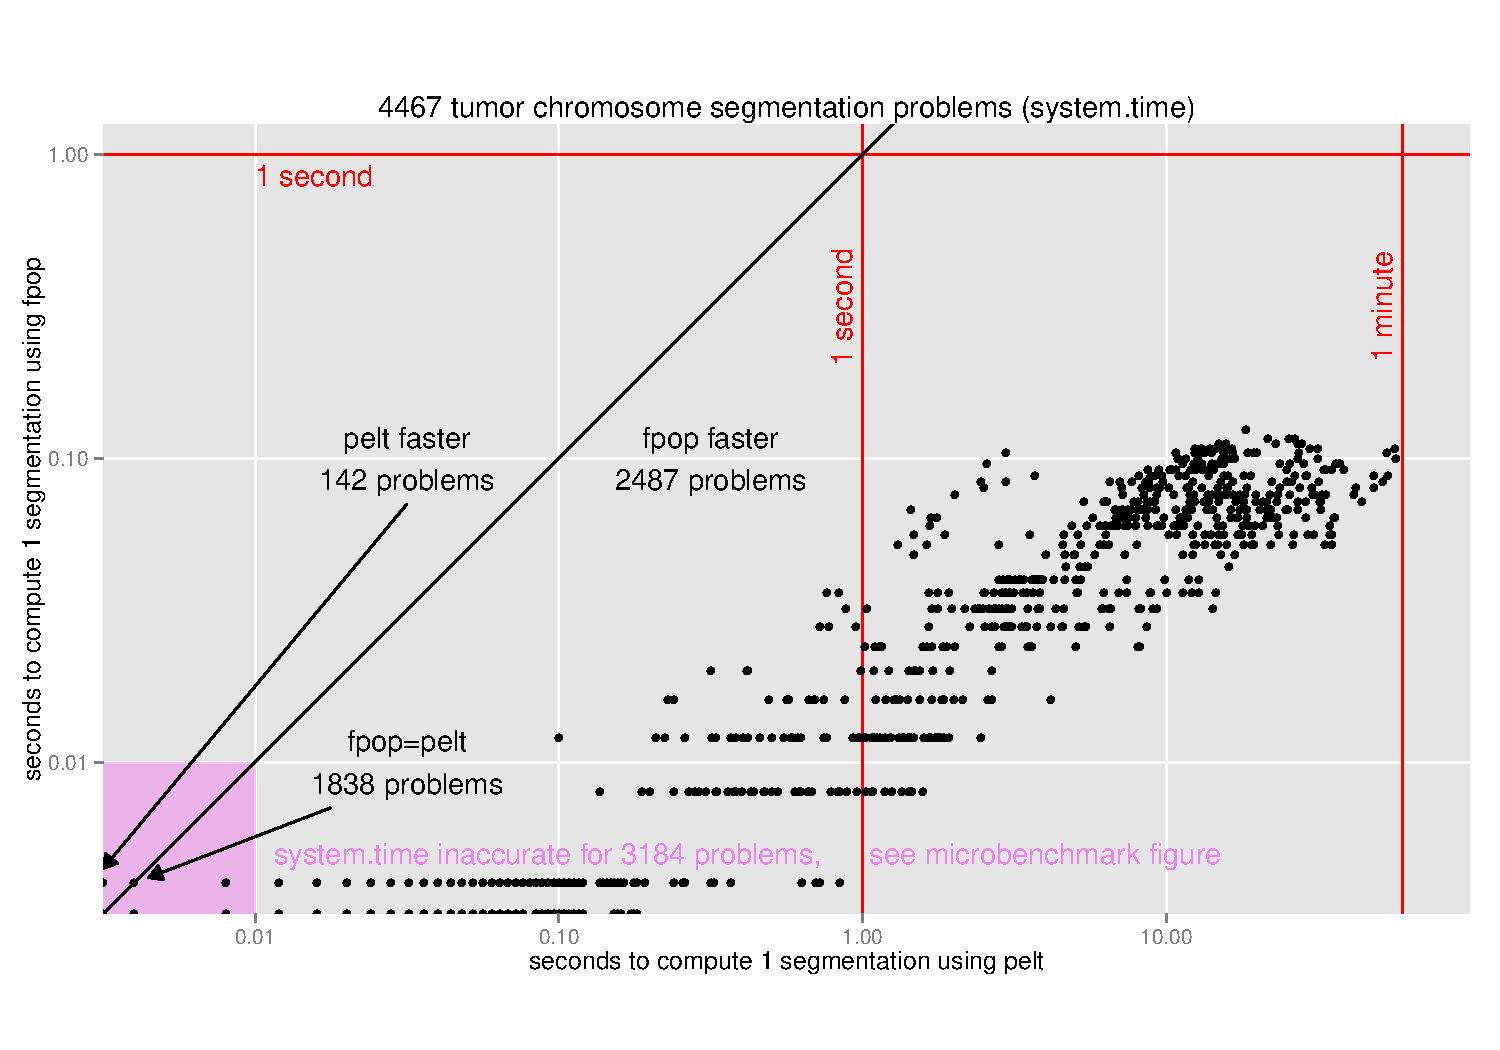
\includegraphics[width=\textwidth]{figure-systemtime-arrays-fpop-pelt}
\end{center}

The plot above shows that fpop is strictly faster than pelt for each
of the segmentation problems. 

\begin{center}
  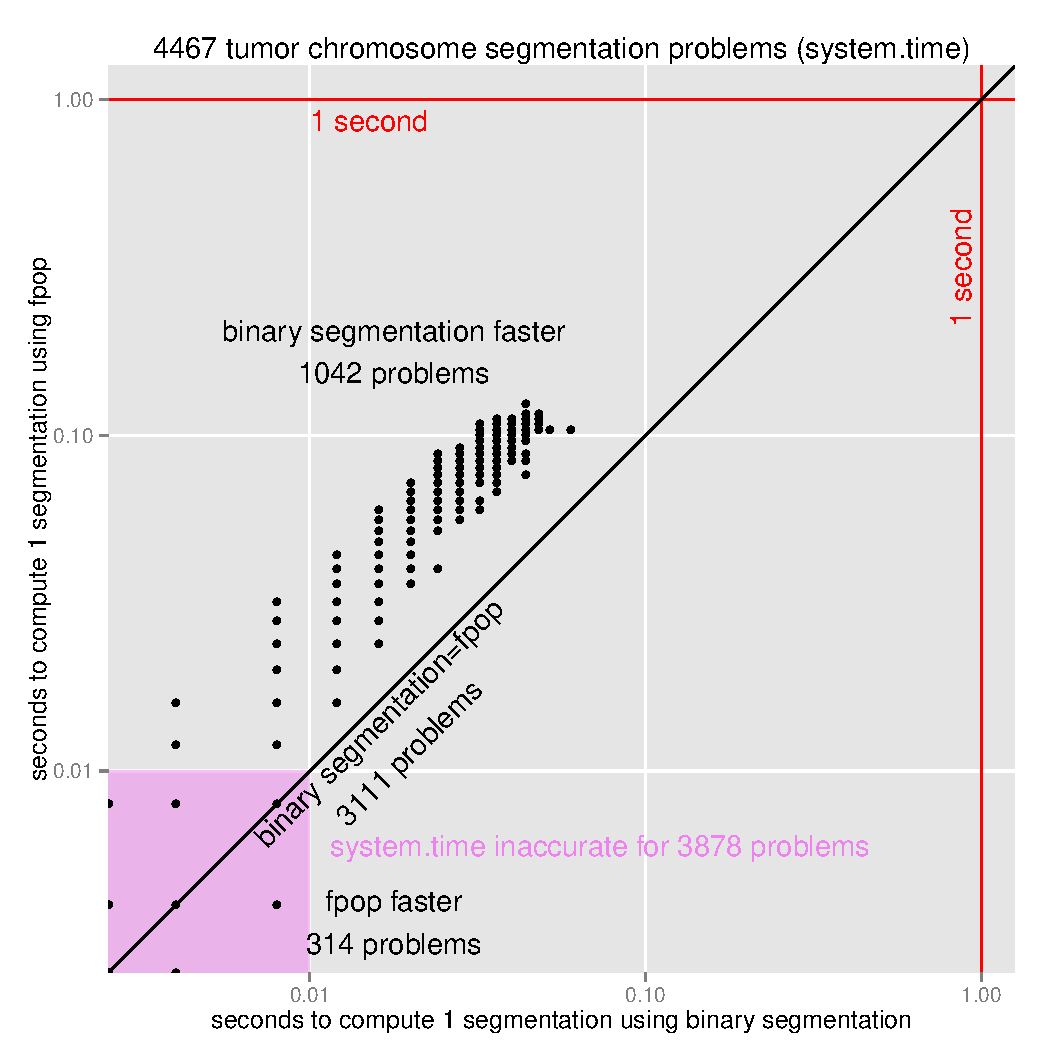
\includegraphics[width=\textwidth]{figure-systemtime-arrays-fpop-multiBinSeg}
\end{center}

The plot above shows that fpop is strictly slower than binary
segmentation for each of the segmentation problems.

\subsection{Timings using microbenchmark in R}

In this section, we used the R \verb|microbenchmark| function to
measure the execution time of fpop, pelt, and binseg on only the small
segmentation problems for which \verb|system.time| was inaccurate. The
R source code for these timings is in
\verb|benchmark/microbenchmark.arrays.R| in the opfp project
repository on R-Forge:

\url{https://r-forge.r-project.org/projects/opfp/}


\begin{center}
  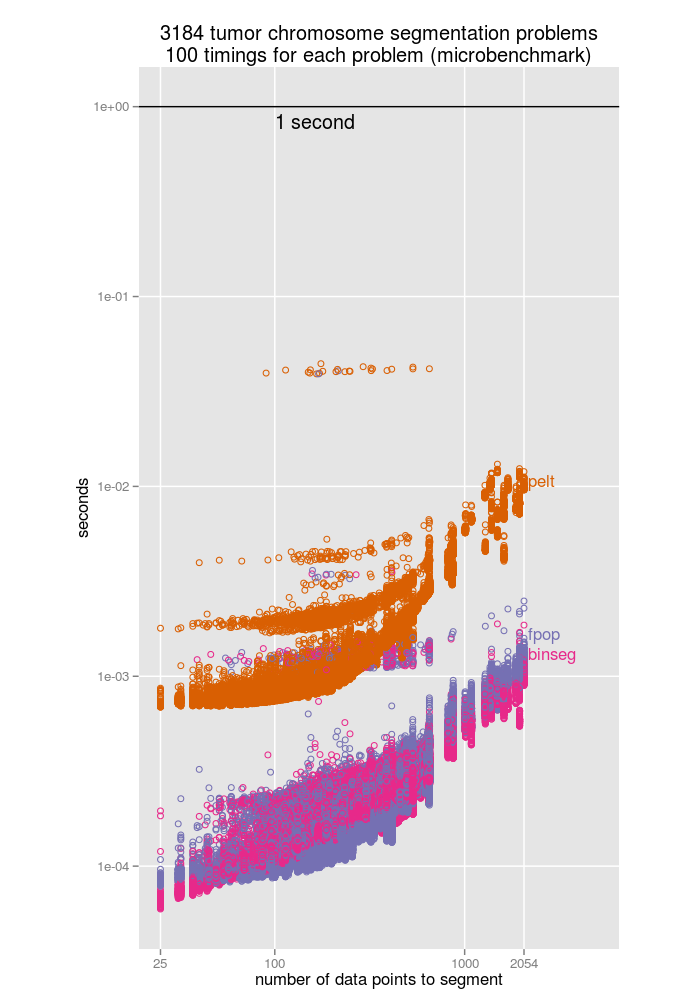
\includegraphics[width=5in]{figure-microbenchmark-arrays}
\end{center}

The figure above shows that in general fpop is faster than pelt but
slower than binseg.

\begin{center}
  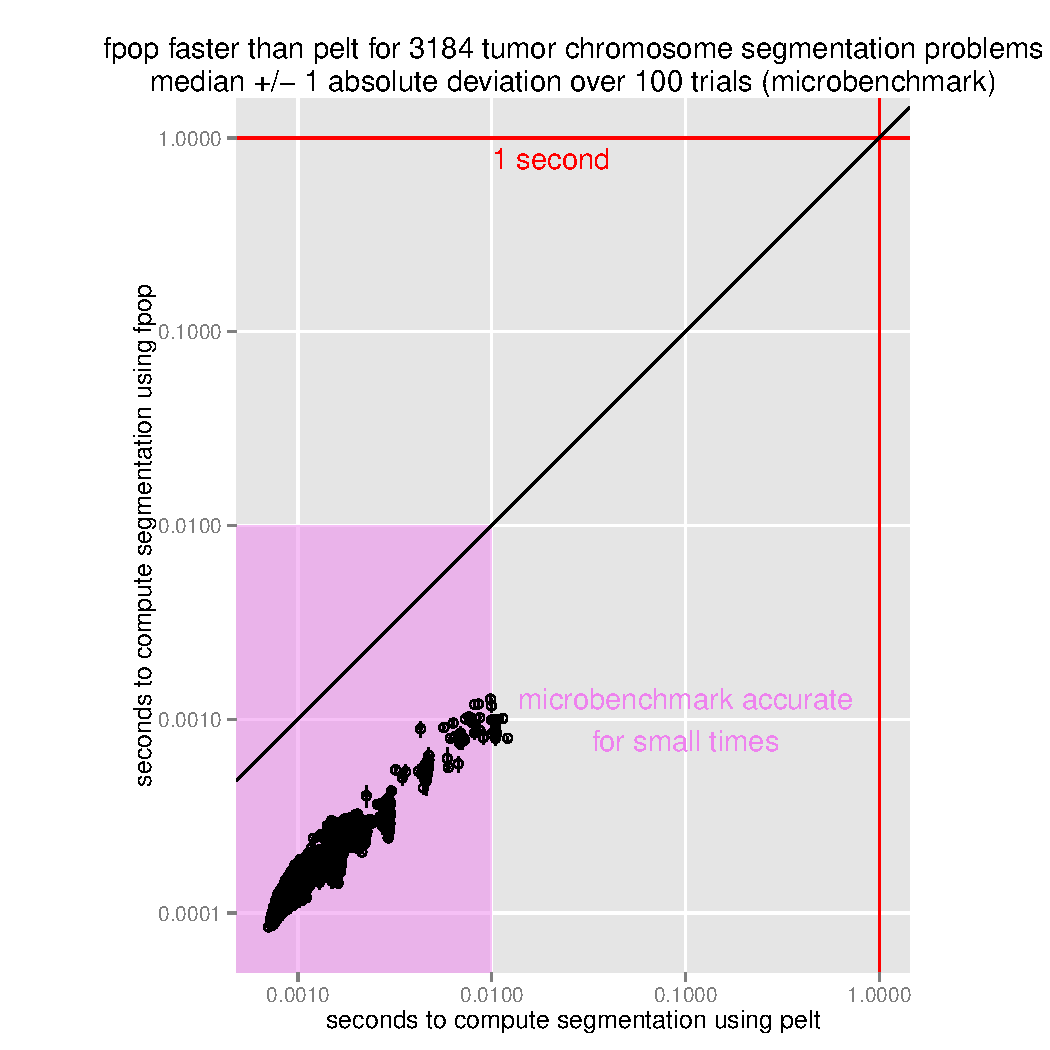
\includegraphics[width=\textwidth]{figure-microbenchmark-arrays-fpop-pelt}
\end{center}

The figure above shows that fpop is strictly faster than pelt for each
segmentation problem.

\begin{center}
  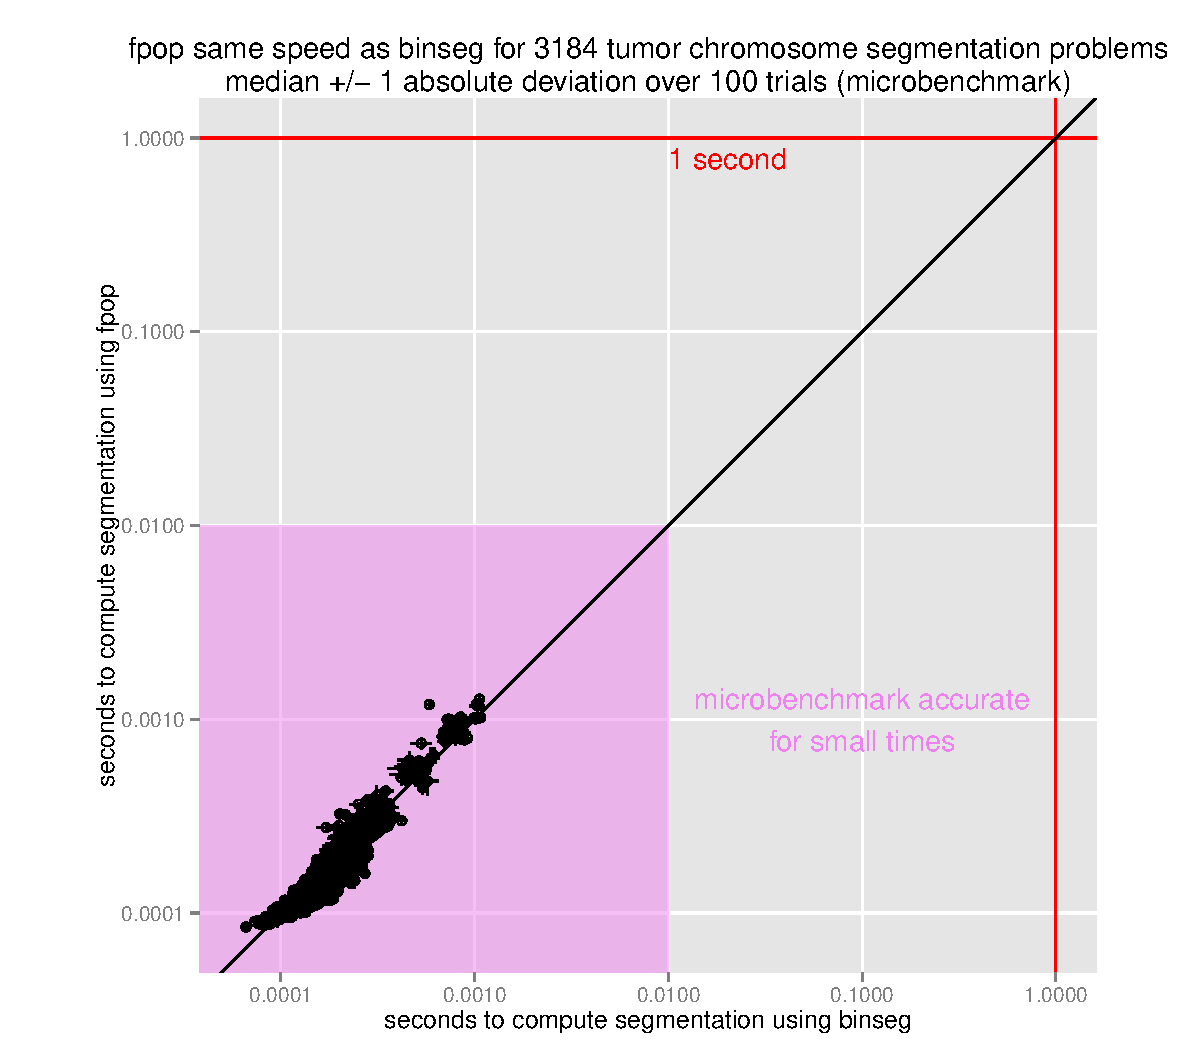
\includegraphics[width=\textwidth]{figure-microbenchmark-arrays-fpop-binseg}
\end{center}

The figure above shows that fpop is about the same speed as binseg for
each of the small segmentation problems with between 25 and 2054 data
points.


\newpage

\section{Speed benchmark: simulated data with different 
  number of changes}

We varied the number of changes in a signal with 200000 data points,
and timed the algorithms for each of these signals. The R source code
for these timings is in \verb|benchmark/systemtime.simulation.R| in
the opfp project repository on R-Forge:

\url{https://r-forge.r-project.org/projects/opfp/}

\begin{center}
  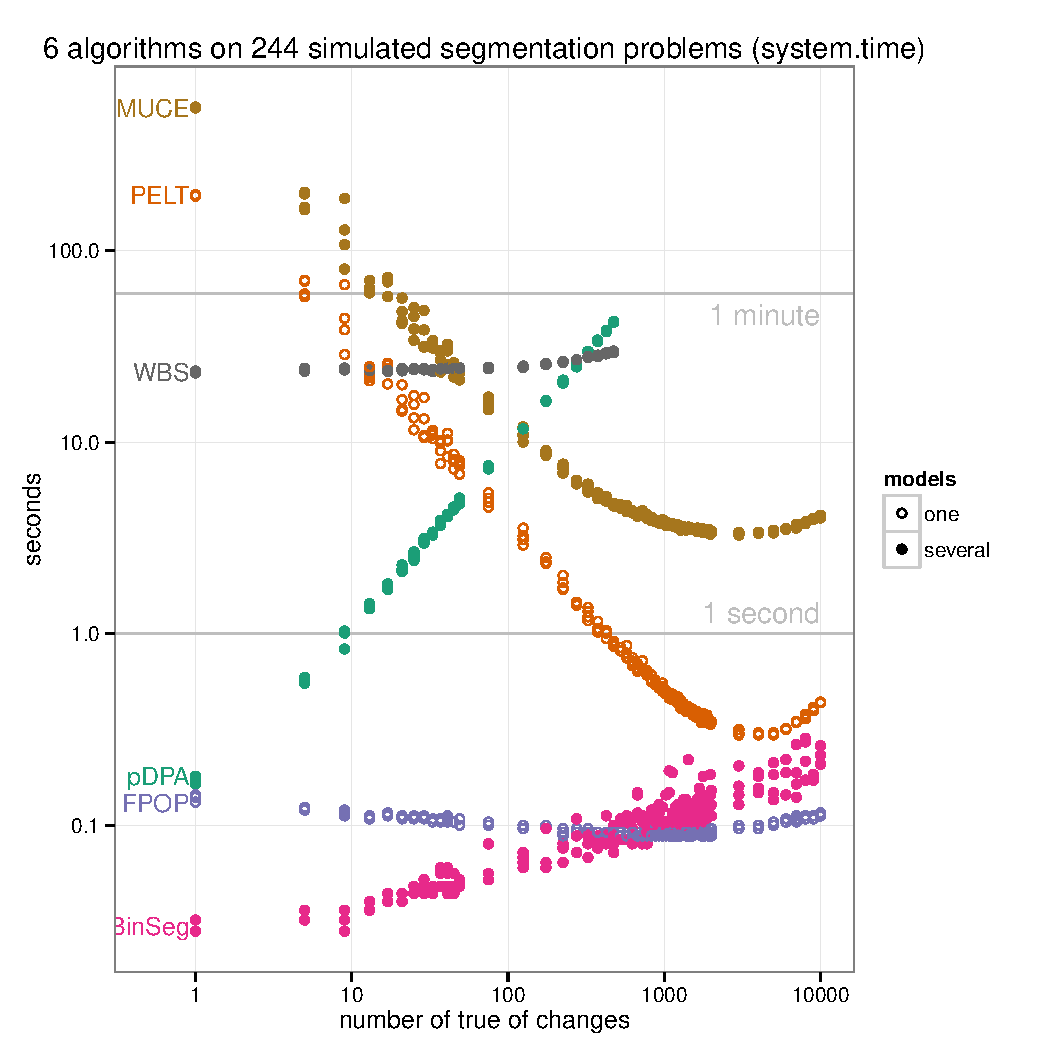
\includegraphics[width=\textwidth]{figure-systemtime-simulation}
\end{center}

It is clear from the figure above that fpop is always faster than
pelt, and that its advantage is bigger for data with few true changes.

\newpage

\section{Appendix: computer system information}

\begin{verbatim}
thocking@silene:~/R/opfp/benchmark$ cat /proc/cpuinfo|grep 'model name'|head -1
model name	: Intel(R) Core(TM) i7 CPU         930  @ 2.80GHz
\end{verbatim}

\bibliographystyle{abbrvnat}
\bibliography{refs}

\end{document}
